\documentclass[xcolor=svgnames, colorlinks, handout]{beamer}
%\documentclass[xcolor=svgnames, handout]{beamer}

%\includeonlyframes{current}

\usepackage[utf8]    {inputenc}
\usepackage[T1]      {fontenc}
\usepackage[english] {babel}

\usepackage{amsmath,amsfonts,graphicx}
\usepackage{beamerleanprogress}
\usepackage{xcolor}
\usepackage{soul}
%\usepackage{verbatim}
\usepackage{multicol}
\usepackage{tikz} 
\usepackage[export]{adjustbox}
\usepackage{array}
\usepackage{fancyvrb}


%%%% https://www.overleaf.com/learn/latex/LaTeX_Graphics_using_TikZ:_A_Tutorial_for_Beginners_(Part_3)%E2%80%94Creating_Flowcharts
\usepackage{tikz}
\usetikzlibrary{shapes.geometric, arrows}

\tikzstyle{startstop} = [rectangle, rounded corners, minimum width=2cm, minimum height=0.75cm,text centered, draw=black, fill=red!30]

\tikzstyle{io} = [rectangle, minimum width=2cm, minimum height=1cm, text centered, draw=black, fill=blue!30]

\tikzstyle{process} = [rectangle, minimum width=2cm, minimum height=0.75cm, text centered, draw=black, fill=orange!30]
\tikzstyle{decision} = [diamond, minimum width=2cm, minimum height=1cm, text centered, draw=black, fill=green!30]

\tikzstyle{arrow} = [thick,->,>=stealth]
%%%%%%%%%%%%%%


%%%%%%%%%%%%%% https://tex.stackexchange.com/questions/274280/building-a-flow-chart-in-beamer-using-tikz

\usetikzlibrary{shapes.geometric, arrows,chains}
\tikzset{
%  startstop/.style={
%    rectangle, 
%    rounded corners,
%    minimum width=3cm, 
%    minimum height=1cm,
%    align=center, 
%    draw=black, 
%    fill=red!30
%    },
%  process/.style={
%    rectangle, 
%    minimum width=3cm, 
%    minimum height=1cm, 
%    align=center, 
%    draw=black, 
%    fill=blue!30
%    },
  decision/.style={
    diamond, 
    minimum width=3cm, 
    minimum height=1cm, align=center, 
    draw=black, 
    fill=green!30
    },
  arrow/.style={thick,->,>=stealth},
  dec/.style={
    ellipse, 
    align=center, 
    draw=black, 
    fill=green!30
    },
}

%%%%%%%%%%%%%%

% https://tex.stackexchange.com/questions/182476/how-do-i-center-a-boxed-verbatim/182479
\newsavebox{\FVerbBox}
\newenvironment{FVerbatim}
 {\VerbatimEnvironment
  \begin{center}
  \begin{lrbox}{\FVerbBox}
  \begin{BVerbatim}}
 {\end{BVerbatim}
  \end{lrbox}
  \fbox{\usebox{\FVerbBox}}
  \end{center}}
  

\setbeamertemplate{theorems}[numbered] 
 
\definecolor{iyellow}{RGB}{255, 162, 23}
\definecolor{sgreen}{RGB}{118, 191, 138}

\newcommand{\yellow}[1]{\textcolor{iyellow}{#1}}
\newcommand{\red}[1]{\textcolor{red}{#1}}
\newcommand{\green}[1]{\textcolor{ForestGreen}{#1}}
\newcommand{\blue}[1]{{\textcolor{blue}{#1}}}
\newcommand{\purple}[1]{{\textcolor{purple}{#1}}}
\newcommand{\orange}[1]{{\textcolor{orange}{#1}}}
\newcommand{\bblue}[1]{\textcolor{SteelBlue!90!gray}{#1}} % beamer blue
\newcommand{\tans}[2]{\textbf<#1>{\textit<#1>{{\color<#1>{iyellow}{#2}}}}}

\newcommand{\eol}{\\[1em]\pause}
\newcommand{\nl}{\\[1em]}
\newcommand{\define}[1]{\textbf{\textcolor{orange}{#1}}}
\newcommand{\answer}[1]{\textit{\textbf{\textcolor{iyellow}{#1}}}}
\newcommand{\command}[1]{\texttt{\textbf{\textcolor{DarkMagenta}{#1}}}}
\newcommand{\ipic}[2]{\includegraphics[width={#2}\textwidth]{#1}}
\newcommand{\cell}[1]{{\sf \textbf{\textcolor{DarkMagenta}{#1}}}}
\newcommand{\ra}{$\rightarrow$}

\newenvironment{allintypewriter}{\ttfamily}{\par}
\newcommand{\ft}[1]{\frametitle{#1}}
\usepackage{fancyvrb}

\usepackage{upquote,textcomp}

\newcommand{\bs}{$\backslash$}

\usepackage[T1]{fontenc}
\usepackage[utf8]{inputenc}
\usepackage{tikz}
\usetikzlibrary{shadows}

\newcommand*\keystroke[1]{%
  \tikz[baseline=(key.base)]
    \node[%
      draw,
      fill=white,
      drop shadow={shadow xshift=0.25ex,shadow yshift=-0.25ex,fill=black,opacity=0.75},
      rectangle,
      rounded corners=2pt,
      inner sep=1pt,
      line width=0.5pt,
      font=\scriptsize\sffamily
    ](key) {#1\strut}
  ;
}

\title
  [Data 301 Data Analytics\hspace{2em}]
  {Data 301 Data Analytics\\
Python Flow Control}

\author
  [Dr.\ Irene Vrbik]
  {Dr.\ Irene Vrbik}

\date
  {Term 1, 2018}

\institute
  {University of British Columbia Okanagan \newline irene.vrbik@ubc.ca}


\graphicspath{{img/}}

\begin{document}

\maketitle

\setbeamersize{description width=0.57cm} % to have less indent with the description environment


\setcounter{theorem}{15}

\begin{frame}[fragile]{Decisions}
\begin{itemize}
% https://www.tutorialspoint.com/cprogramming/c_decision_making.htm
\item \define{Decisions} are used in programming to
specify one or more conditions to be tested, along with statement(s) to  execute if the condition is true.\nl

\item A \define{condition} is an expression that is either {\tt True} or {\tt False}.\nl

\item These conditions control the flow of you program and different statements will be carried out depending on the outcome of these conditions.\nl

\item To build conditional statements we need to be able to write \emph{Boolean expressions}.


\end{itemize}
\end{frame}

\begin{frame}[fragile]{Boolean Expressions}
\begin{itemize}
\item A \define{Boolean expression} is an expression that evaluates to a \emph{Boolean value}\footnote{\noindent The name comes from \href{https://en.wikipedia.org/wiki/George_Boole}{George Boole}, who first defined an algebraic system of logic in the mid 19th century} .
\medskip
\item A \define{Boolean value} is  either {\tt True} or {\tt False}.
\end{itemize}
\begin{alertblock}{Boolean values}
Boolean values are \textit{not} strings. The Python type for storing {\tt True} and {\tt False} values is called {\tt bool}.
\begin{verbatim}
>>> print(type(True)) 
<class 'bool'>
>>> print(type("True"))
<class 'str'>
\end{verbatim}
\end{alertblock}
\end{frame}

\begin{frame}[fragile]{Boolean Expressions}
We can create Boolean expressions using:
\begin{description}
\item[Relational operators/Comparisons:] used to compare two values 
%\begin{itemize}
%\item less-than ({\tt <}) and greater-than ({\tt >})
%\item less-than equal to ({\tt $\leq$}) and greater-than equal to ({\tt $\geq$})
%\item Equals ({\tt ==}), not equals ({\tt !=})\nl
%\end{itemize}
\begin{itemize}
\item Examples:
\begin{verbatim}
5 < 10  # returns True
N > 5   # N is a variable. Answer depends on N.
\end{verbatim}
\end{itemize}
\vspace{1em}
\item[Logical operators:] the logical operators  \blue{\tt and}, \blue{\tt or} and \blue{\tt not} are used to combine relational operators.
\begin{itemize}
\item Example:
\begin{allintypewriter}
(n > 5) \blue{\tt and} (v != n)
\end{allintypewriter}
\vspace{1em}
\end{itemize}
\end{description}
The result these expressions are a \emph{Boolean value} which is either {\tt True} or {\tt False}.
\end{frame}



\begin{frame}[fragile]\ft{Comparisons}

A \define{condition} is a Boolean expression that is either {\tt True} or {\tt False} and may contain one or more comparisons.\nl

The comparison operators in Python are summarized below:
\begin{center}
\begin{tabular}{| >{\ttfamily}c | l  |}\hline
 {\bf Syntax} & {\bf Description} \\\hline
>	&	 Greater than\\
>=	&	 Greater than or equal\\
< 	&	 Less than\\
<=	&	  Less than or equal\\
==	&	  Equal (Note: Not "=" which is used for assignment!)\\
!=	&	  Not equal \\
\hline
\end{tabular}
\end{center}
\end{frame}

\begin{frame}[fragile]\ft{Conditions with {\tt and, or, not}}
  Conditions may be combined using the relational operators \blue{\tt and, or, not.}\nl
\begin{center}
\begin{tabular}{ |l  | >{\ttfamily}c | >{\ttfamily}c | >{\ttfamily}c |}\hline
 {\bf True if:} & {\bf Syntax} & {\bf Examples}& {\bf Outpu} \\\hline
both are true 	& \blue{and} & \green{True} \blue{and} \green{True}& \green{True}\\
&& \red{False} \blue{and} \green{True} & \red{False} \\\hline
either or both are T 	& \blue{or} &	 \green{True} \blue{or} \green{True} & \green{True}\\
&& \red{False} \blue{or} \green{True} & \green{True}\\
&& \red{False} \blue{or} \red{False} & \red{False}\\\hline
false	& \blue{not} &	\blue{not} \green{True} & \red{False}	 \\
&& \blue{not} \red{False} & \green{True} \\\hline
\end{tabular}
\end{center}
\end{frame}

\begin{frame}[fragile]\ft{Condition Examples}
%\begin{verbatim}
%n = 5
%v = 8
%print(n > 5)				# False
%print(n == v)				# False
%print(n != v)				# True
%print(n == v and n+4>v)		# False
%print(n == v or n+4>v)		# True
%print(n+1 == v-2 or not v>4)	# True
%\end{verbatim}
\begin{allintypewriter}
n = 5 \newline
v = 8\newline
print\red{(n > 5)} \#False \newline
print\red{(n == v)} \#False \newline
print\green{(n != v)} \# True\newline
print(\red{(n == v)} \blue{and} \green{(n+4>v)}) \# False\newline
print(\red{(n == v)} \blue{or} \green{(n+4>v)}) \# True\newline
print(\green{(n+1) == (v-2)} \blue{or} \red(\blue{not} \green{v>4}\red)) \# True\newline
print(\green{(n+1) == (v-2) or not v>4)} \blue{and} \red{(n>5)}) \# False\newline
\end{allintypewriter}
\end{frame}

\begin{frame}{Order of Operations}
\begin{table}[htdp]
\caption{The order of operations; see complete list   \href{https://en.wikipedia.org/wiki/Order\_of\_operations\#Programming_languages}{here}.}
%Order of evaluation: {\tt not, and, or}. May change order with parentheses.
\begin{center}
\begin{tabular}{|c|l|}
\hline
{\tt ()} & brackets\\
{\tt **} & exponents\\
{\tt 	*   /   \% MOD } & Multiplication, division, modulo \\
{\tt 	+ -  } & Addition and subtraction \\
{\tt <   <=   >   >=}	& Comparisons: less-than and greater-than\\
{\tt ==   !=} & 	Comparisons: equal and not equal\\
\blue{\tt and} & and \\
\blue{\tt or} & or \\
\hline
\multicolumn{2}{|c|}{\blue{\tt not}s always bind to the condition immediate next to it}\\
\hline
\end{tabular}
\end{center}
\label{default}
\end{table}%

\begin{block}{Tip:}
I recommend  always using brackets to avoid confusion.
\end{block}


\end{frame}


%%%%%%%%%%%%%%%%%%%%%%%%%

% question:

\begin{frame}[fragile]\ft{}
  \begin{example}
How many of the following conditions are TRUE?

\begin{enumerate}
\item {{True and False}}
\item {{not True or not False}} 
\item {{\tt 3 + 2 == 5 or 5 > 3 and 4 != 4}}  
\item {{\tt (1 < 2 or 3 > 5) and (2 == 2 and 4 != 5)}} 
\item {\tt not (True or False) or True and (not False)}
\end{enumerate}
\begin{multicols}{5}
\begin{enumerate}[A)]
\item 1
\item 2
\item 3
\item 4
\item 5
\end{enumerate}
\end{multicols}
  \end{example} 
\end{frame}


% answer:

\begin{frame}<handout:0>[fragile]\ft{}
  \begin{block}{Answer:}
How many of the following conditions are TRUE?
\begin{enumerate}
\item {\color<1->{red}	{True and False}} = \green{\tt True} \blue{\tt or} \red{\tt False}
\item {\color<2->{sgreen}	{not True or not False}} = {\tt \red{(not True)} or \green{(not False)}}
\item {\color<3->{sgreen}	{\tt 3 + 2 == 5 or 5 > 3 and 4 != 4}}\newline
= {\tt \green{(5 == 5)} or \green{(5 > 3)} and \red{(4 != 4)}}\newline
= {\tt \green{(5 == 5)} or \red{((5 > 3) and (4 != 4))}} \# and first
\item {\color<4->{sgreen}	{\tt (1 < 2 or 3 > 5) and (2 == 2 and 4 != 5)}} \newline
{\tt (\green{1 < 2} or \red{3 > 5}) {and} \green(\green{2 == 2} {and} \green{4 != 5}\green)}\newline
{\tt \green{({1 < 2} or \green{3 > 5}\green)} and \green{(\green{2 == 2} and \green{4 != 5}\green)}}
\item {\color<5->{sgreen}	{\tt not (True or False) or True and (not False)}}\newline
{\tt not \green{(True or False)} or True and \green{(not False)}}\newline
{\tt \red{not {(True or False)}} or \green{True and \green{(not False)}}}\newline
\end{enumerate}
\begin{multicols}{5}
\begin{enumerate}[A)]
\item 1
\item 2
\item 3
\item \tans{5}{4} 
\item 5
\end{enumerate}
\end{multicols}
  \end{block} 
\end{frame}
%%%%%%%%%%%%%%%%%%%%%%%%%

\begin{frame}[fragile]\ft{Decisions}
%\define{Decisions} allow the program to perform different actions based on  conditions. 
In Python decision syntax:
\ipic{if}{0.9}
\begin{itemize}
\item The statement(s) after the \define{\tt if} condition  is only performed if the \command{\it condition} (i.e. Boolean expression) returns  {\tt True}.
\item Any statement(s) following the (optional) \define{\tt else:} condition is only performed if the \command{\it condition} is {\tt False}.
\end{itemize}
\begin{alertblock}{Python syntax}
Remember that the indentation and colons are \textit{not} optional! 
\end{alertblock}

\end{frame}


\begin{frame}[fragile]\ft{Decision Block Syntax}
\begin{itemize}
\item Statements listed after an {\tt if}/{\tt esleif}/{\tt esle} clause  are not only indented for readability. \nl
\item These indentation is also how Python knows which statements are part of the group of statements to be executed.\nl
\item Statements with the same indentation belong to the same group called a \define{suite}.\nl
\item %If you have more than one statement, make sure to indent them.  
Be consistent with either using tabs or spaces (no mixing)
\end{itemize}
\begin{block}{Tip: one-line if clause}
If the suite of an if clause consists of a single line, it may go on the same line as the header statement.
\begin{verbatim}
if (n > 100): print("n is large")
\end{verbatim}

\end{block}
%\begin{itemize}
%\item
%\begin{verbatim}
%if age > 19 and name > "N":
%    print("Not a teenager")
%    print("Name larger than N")
%else:
%    print("This is statement #1")
%    print(" and here is statement #2!")
%\end{verbatim}
%\end{itemize}
\end{frame}



\begin{frame}[fragile]\ft{Decisions if/elif Syntax}
Check out the difference for {\tt age = 20}:
\begin{columns}[T] % align columns
\begin{column}{.4\textwidth}
\begin{Verbatim}
age = 20
if age > 19:
    print("Not a teenager")
    print("Sorry")
else:
    print("You're young")
    print("ID checked")
\end{Verbatim}
The above returns:
\begin{Verbatim}[frame=single]
Not a teenager
Sorry
\end{Verbatim}
\end{column}%

\begin{column}{.4\textwidth}
\begin{Verbatim}
age = 20
if age > 19:
    print("Not a teenager")
    print("Sorry")
else:
    print("You're young")
print("ID checked")
\end{Verbatim}
The above returns:
\begin{Verbatim}[frame=single]
Not a teenager
Sorry
ID checked
\end{Verbatim}

\end{column}%
\end{columns}
\end{frame}
%Note: No switch statement like other languages but there are approaches based on dictionaries (hash tables) that can be used.




\begin{frame}[fragile]

\begin{columns}[T] % align columns
\begin{column}{.3\textwidth}
Generic code:
\begin{Verbatim}[frame=single]
if (cond1):
    Process 1
\end{Verbatim}
\vspace{1em}
Example 1:
\begin{Verbatim}[frame=single]
n = 5
if (n < 10):
    n = 10
\end{Verbatim}
{\tt n} is now {\tt 10}\\
\vspace{1em}
Example 2:
\begin{Verbatim}[frame=single]
n = 5
if (n > 10):
    n = 10
\end{Verbatim}
{\tt n} remains {\tt 5}

\end{column}%

\begin{column}{.5\textwidth}
\begin{center}
 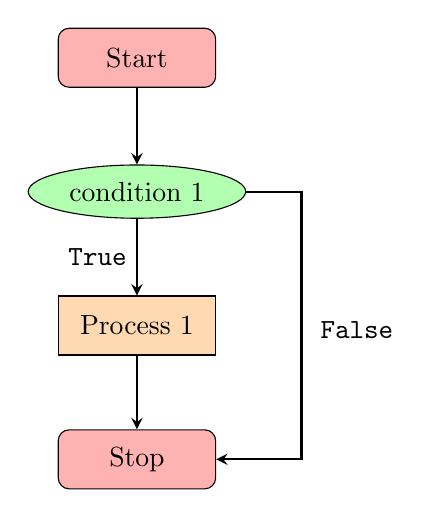
\begin{tikzpicture}[
  start chain=going below,
  every join/.style={arrow},
  node distance=1.7cm
  ]
\node (start) [startstop] {Start};
\node (cond1) [dec, below of = start] {condition 1};
\node (state1) [process,below of=cond1] {Process 1};
\node (stop) [startstop, below of=state1] {Stop};
%\node (np) [io, below of=stop] {New Process};

\draw [arrow] (start) -- (cond1);
\draw [arrow] (cond1) -- node[anchor=east] {{\tt True}}(state1);
\draw [arrow] (state1) -- (stop);
\draw[arrow] (cond1.east) -- node[xshift = 3em, yshift=- 5em] {\tt False} ++(20pt,0pt) |- (stop.east);
%\draw [arrow] (stop) -- (np);

\end{tikzpicture}%
%}
\end{center}
\end{column}%
\end{columns}
\end{frame}


\begin{frame}[fragile]

\begin{columns}[T] % align columns
\begin{column}{.3\textwidth}
Generic code:
\begin{Verbatim}[frame=single]
if (cond1):
    Process 1
else:
    Process 2
\end{Verbatim}
\vspace{1em}
Example :
\begin{Verbatim}[frame=single]
n = 5
if (n > 10):
    n = 10
else:
    n = 3
\end{Verbatim}
{\tt n} is now {\tt 3}
\end{column}%

\begin{column}{.5\textwidth}
\begin{center}
 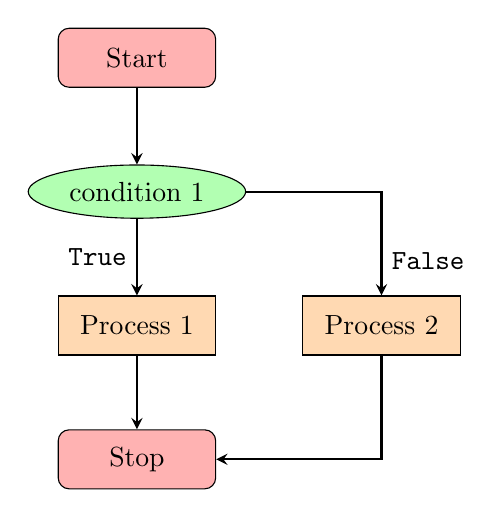
\begin{tikzpicture}[
  start chain=going below,
  every join/.style={arrow},
  node distance=1.7cm
  ]
\node (start) [startstop] {Start};
\node (cond1) [dec, below of = start] {condition 1};
\node (state1) [process,below of=cond1] {Process 1};
\node (state2) [process,right of=state1, xshift = 4 em] {Process 2};
\node (stop) [startstop, below of=state1] {Stop};
%\node (np) [io, below of=stop] {New Process};

\draw [arrow] (start) -- (cond1);
\draw [arrow] (cond1) -- node[anchor=east] {{\tt True}}(state1);
\draw [arrow] (state1) -- (stop);
\draw [arrow] (cond1) -| node[anchor=west, yshift = -2.5em] {{\tt False}}(state2);
\draw [arrow] (state2) |- (stop);
\end{tikzpicture}%
%}
\end{center}
\end{column}%
\end{columns}
\end{frame}












\begin{frame}[fragile]\ft{Decisions if/elif Syntax}
If there are more than two choices, use {\tt if/elif/else} statements.  \alert{N.B. once a condition is met, no subsequent conditions are checked}
\vspace{-1em}
\begin{columns}[T] % align columns
\begin{column}{.4\textwidth}
\begin{Verbatim}[frame=single]
if condition1:
    Process 1
elif condition2:
    Process 2
elif condition3:
    Process 3
else:
    Process 4
\end{Verbatim}
\end{column}%

\begin{column}{.4\textwidth}
\begin{Verbatim}[frame=single]
if n == 1:
    print("one")
elif n == 2:
    print("two")
elif n == 3:
    print("three")
else:
    print("Too big!")
print("Done!")
\end{Verbatim}
\end{column}%
\end{columns}
\begin{block}{\tt else}
Again, the {\tt else} statement is an optional. There could be at most one {\tt else} statement following an {\tt if}.
\end{block}
\end{frame}
%Note: No switch statement like other languages but there are approaches based on dictionaries (hash tables) that can be used.


\begin{frame}[fragile]{\tt if, elif, else}
\begin{center}
 \begin{tikzpicture}[
  start chain=going below,
  every join/.style={arrow},
  node distance=1.5cm
  ]
%\node (start) [startstop] {Start};
\node (cond1) [dec, below of = start] {condition 1};
\node (state1) [process, below of = cond1] {Process 1};
\node (cond2) [dec, below of = cond1, right of = cond1, xshift=3em] {condition 2};
\node (state2) [process, below of = cond2] {Process 2};
\node (cond3) [dec, below of = cond2, right of = cond2, xshift=3em] {condition 3};
\node (state3) [process, below of = cond3] {Process 3};
%\node (cond4) [dec, below of = cond3, right of = cond3, xshift=3em] {condition 4};
\node (state4) [process, below of = state3, right of = state3, xshift = 2em] {Process 4};
\node (stop) [startstop, below of = cond2, yshift=-10em] {Stop};

%\draw [arrow] (start) -- (cond1);
\draw [arrow] (cond1) -- node[anchor=east] {{\tt True}}(state1);
\draw [arrow] (cond2) -- node[anchor=east] {{\tt True}}(state2);
\draw [arrow] (cond3) -- node[anchor=east] {{\tt True}}(state3);
\draw [arrow] (cond3) -| node[anchor=east, xshift = 4em, yshift = -4em  ] {{\tt False}}(state4);
\draw [arrow] (state1) |- (stop);
\draw [arrow] (state2) -- (stop);
\draw [arrow] (state3) |- (stop);
\draw [arrow] (state4) |- (stop);

\draw [arrow] (cond1) -| node[anchor=west, yshift = -2em] {{\tt False}}(cond2);
\draw [arrow] (cond2) -| node[anchor=west, yshift = -2em] {{\tt False}}(cond3);
%\draw [arrow] (cond3) -| node[anchor=west, yshift = -2.2em] {{\tt False}}(cond4);
\end{tikzpicture}


\end{center}
\end{frame}





\begin{frame}[fragile]\ft{Decisions if/elif Syntax}

\begin{Verbatim}[frame=single,numbers=left]
n = 1
if n == 1:
    print("one")
elif n>0: # this condition is never checked since the
    # condition on line 2 has already been satisfied
    print("positive number")
elif n == 3:
    print("three")
else:
    print("Too big!")
print("and Done!") #  not part of the if statement
\end{Verbatim}
The above returns:
\begin{Verbatim}[frame=single]
one
and Done!
\end{Verbatim}

\end{frame}


\begin{frame}[fragile]\ft{Decisions if/elif Syntax}
\begin{Verbatim}[frame=single,numbers=left]
n = 3
if n == 1:
    print("one")
elif n>0: 
    print("positive number")
elif n == 3: # this condition is never checked since 
    # condition on line 4 has already been satisfied
    print("three")
else:
    print("Too big!")
print("and Done!") #  not part of the if statement
\end{Verbatim}
The above returns:
\begin{Verbatim}[frame=single]
positive number
and Done!
\end{Verbatim}

\end{frame}





\begin{frame}[fragile]\ft{Decisions Multiple {\tt if} statements}
\begin{itemize}
\item  As mentioned previously, once a condition is met in an if/elif statement, no subsequent conditions are checked. \nl
\item If we want all conditions to be checked we could use multiple {\tt if} statements:
\end{itemize}
\vspace{-1.5em}
\begin{columns}[T] % align columns
\begin{column}{.3\textwidth}
\begin{Verbatim}[frame=single]
if condition1:
    Process 1
if condition2:
    Process 2
if condition3:
    Process 3
if condition4:
    Process 4
\end{Verbatim}
\end{column}%
\begin{column}{.55\textwidth}
\begin{Verbatim}[frame=single]
n = 3
if n > 0: 
    print("positive number")
if n == 3: 
    print("three")
if n < 10:
    print("single digit")
\end{Verbatim}
$\uparrow$ returns $\rightarrow$
\vspace{-2em}
\begin{Verbatim}[xleftmargin=0.8in, frame=single]
positive number
three
single digit
\end{Verbatim}

\end{column}%
\end{columns}
\end{frame}







%%%%%%%%%%%%%%%%%%%%%%%%

% question:

\begin{frame}[fragile]\ft{}
  \begin{example}
What is the output of the following code?
\begin{verbatim}
    n = 3
    if n < 1:
        print("one")
    elif n > 2:
        print("two")
    elif n == 3:
        print("three")
\end{verbatim}

\begin{enumerate}[A)]
\item {{nothing}}
\item {{one}}
\item {{two}}
\item {{three}} 
\item {{error}}
\end{enumerate}
  \end{example} 
\end{frame}


% answer:

\begin{frame}<handout:0>[fragile]\ft{}
  \begin{block}{Answer:}
What is the output of the following code?
\begin{verbatim}
    n = 3
    if n < 1:
        print("one")
    elif n > 2:
        print("two")
    elif n == 3:
        print("three")
\end{verbatim}
\begin{enumerate}[A)]
\item {\color<1->{red}	{nothing}}
\item {\color<1->{red}	{one}}
\item {\color<1->{sgreen}	{two}}
\item {\color<1->{red}	{three}} 
\item {{error}}
\end{enumerate}
  \end{block} 
\end{frame}


%%%%%%%%%%%%%%%%%%%%%%%%%


% question:

\begin{frame}[fragile]\ft{}
  \begin{example}
What is the output of the following code?
\begin{Verbatim}[xleftmargin=0.5in]
n = 3
if n < 1:
    print("one")
elif n > 2
    print("two")
else:
    print("three")
\end{Verbatim}

\begin{enumerate}[A)]
\item {{nothing}}
\item {{one}}
\item {{two}}
\item {{three}} 
\item {{error}}
\end{enumerate}
  \end{example} 
\end{frame}


% answer:

\begin{frame}<handout:0>[fragile]\ft{}
  \begin{block}{Answer:}
What is the output of the following code?
\begin{Verbatim}[xleftmargin=0.5in]
n = 3
if n < 1:
    print("one")
elif n > 2
    print("two")
else:
    print("three")
\end{Verbatim}
\begin{enumerate}
\item {\color<1->{red}	{nothing}}
\item {\color<1->{red}	{one}}
\item {\color<1->{red}	{two}}
\item {\color<1->{red}	{three}} 
\item {\color<1->{sgreen} {error (missing colon)}}
\end{enumerate}
  \end{block} 
\end{frame}


%%%%%%%%%%%%%%%%%%%%%%%%%

% question:

\begin{frame}[fragile]\ft{}
  \begin{example}
What is the output of the following code?
\begin{Verbatim}[xleftmargin=0.5in]
n = 1
if n < 1:
    print("one")
elif n > 2:
    print("two")
else:
    print("three")
print("four")
\end{Verbatim}

\begin{multicols}{5}
\begin{enumerate}[A)]
\item nothing
\item one \newline four
\item three \newline
\item three\newline four
\item error
\end{enumerate}
\end{multicols}
  \end{example} 
\end{frame}


% answer:

\begin{frame}<handout:0>[fragile]\ft{}
  \begin{block}{Answer:}
What is the output of the following code?
\begin{Verbatim}[xleftmargin=0.5in]
n = 1
if n < 1:
    print("one")
elif n > 2:
    print("two")
else:
    print("three")
print("four")
\end{Verbatim}
\begin{multicols}{5}
\begin{enumerate}[A)]
\item nothing
\item one \newline four
\item three \newline
\item \answer{three}\newline \answer{four}
\item error
\end{enumerate}
\end{multicols}
  \end{block} 
\end{frame}


%%%%%%%%%%%%%%%%%%%%%%%%%


% question:

\begin{frame}[fragile]\ft{}
  \begin{example}
What is the output of the following code?
\begin{Verbatim}[xleftmargin=0.5in]
n = 0
if n < 1:
    print("one")
    print("five")
elif n == 0:
    print("zero")
else:
    print("three")
print("four")
\end{Verbatim}
\begin{multicols}{5}
\begin{enumerate}[A)]
\item nothing \newline\newline
\item one \newline four \newline\newline
\item one \newline five \newline four\newline
\item {one}\newline {five} \newline zero \newline four
\item error \newline\newline
\end{enumerate}
\end{multicols}
  \end{example} 
\end{frame}


% answer:

\begin{frame}<handout:0>[fragile]\ft{}
  \begin{block}{Answer:}
What is the output of the following code?
\begin{Verbatim}[xleftmargin=0.5in]
n = 0
if n < 1:
    print("one")
    print("five")
elif n == 0:
    print("zero")
else:
    print("three")
print("four")
\end{Verbatim}
\begin{multicols}{5}
\begin{enumerate}[A)]
\item nothing \newline\newline
\item one \newline four \newline\newline
\item \answer{one} \newline \answer{five} \newline \answer{four}\newline
\item {one}\newline {five} \newline zero \newline four
\item error \newline\newline
\end{enumerate}
\end{multicols}
  \end{block} 
\end{frame}


%%%%%%%%%%%%%%%%%%%%%%%%%

\begin{frame}{Try it: Decisions}
\begin{example}
Write a Python program that asks the user for a number then prints out if it is even or odd.
\end{example}
\begin{example}
Write a Python program that asks the user for an integer.  If that  number is between 1 and 5, prints out the word for that number (e.g. 1 is one).  If the number is not in that range, print out error.
\end{example}
\end{frame}








\begin{frame}[fragile]\ft{Loops and Iteration}
A \define{loop} repeats a set of statements multiple times until some condition is satisfied.
\begin{itemize}
\item Each time a loop is executed is called an \define{iteration}.\nl
\end{itemize}

A \blue{\tt for} loop repeats statements a certain number of times.  
\begin{itemize}
\item It will iterate over a sequence, eg. 1, 2, .\dots 10
\item or it could iterate over group/collection elements, eg. lines in a document, elements in a list \nl
\end{itemize}



A \blue{\tt while} loop repeats statements while a condition is True.
\begin{itemize}
\item At each iteration we will check this condition.
\item If its {\tt True} we complete another iteration
\item If its {\tt False} we exit the loop.
\end{itemize}
\end{frame}

\begin{frame}[fragile]\ft{{\tt while} loops}
The most basic looping structure is the \emph{while} loop.\nl
A while loop continually executes a set of statements while a condition is true.
Syntax:
\begin{center}
\begin{allintypewriter}
\orange{while} condition\orange:
\newline  statement1
\newline  statement2
\newline \vdots
\end{allintypewriter}
\end{center}

 Example:
 \vspace{-2em}
\begin{Verbatim}[xleftmargin=0.8in, frame=single]
n = 1
while n <= 5:
    print(n)
    n = n + 1 
\end{Verbatim}
prints the values 1 through 5.
\end{frame}
%Note: No ++ or -? operators in Python.
%
%Writes 1 to 5.
%
%Something completely different about Python is the�while/else�construction.�while/else is similar to�if/else, but there�is�a difference: the�else�block will execute anytime�the loop condition is evaluated to False. This means that it will execute if the loop is never entered or if the loop exits normally. If the loop exits as the result of a break, the�else�will not be executed.
%In this example, the loop will�break�if a 5 is generated, and the�else�will not execute. Otherwise, after 3 numbers are generated, the loop condition will become false and the else will execute.



\begin{frame}[fragile]{{\tt while} loops}
\begin{center}
 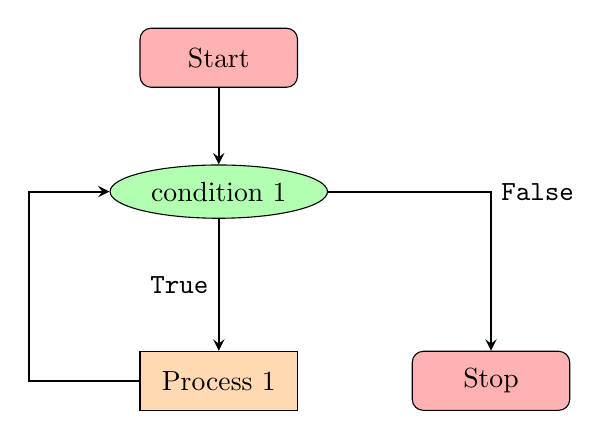
\begin{tikzpicture}[
  start chain=going below,
  every join/.style={arrow},
  node distance=1.7cm
  ]
\node (start) [startstop] {Start};
\node (cond1) [dec, below of = start] {condition 1};
\node (state1) [process,below of=cond1, yshift = -2em] {Process 1};
\node (stop) [startstop, right of =state1, xshift = 5em] {Stop};
%\node (np) [io, below of=stop] {New Process};

\draw [arrow] (start) -- (cond1);
\draw [arrow] (cond1) -- node[anchor=east] {{\tt True}}(state1);
\draw [arrow] (cond1) -| node[anchor=west] {{\tt False}} (stop);
\draw[arrow] (state1.west) --  ++(-40pt,0pt) |- (cond1.west);

\end{tikzpicture}%
%}
\end{center}
\end{frame}


% SHOULD I INCLUDE THIS?
% With the break statement we can stop the loop even if the while condition is true:


\begin{frame}[fragile]{Shorthand}
In addition to the {\tt =} operator for assigning a value to a variable, Python also supports a shorthand version that compounds various  mathematical operators with the assignment operator:
\begin{table}[htdp]
\caption{Table taken from \href{https://www.programiz.com/python-programming/operators}{this} source}
\begin{center}
\begin{tabular}{|c|c|c|}
\hline
{\bf Operator} & {\bf Example} & {\bf Equivalent to} \\
\hline
{\tt =} &	{\tt x = 5} & {\tt 	x = 5}\\
{\tt +=} & 	{\tt x += 5} & 	{\tt x = x + 5} \\
{\tt -=} & 	{\tt x -= 5} & 	{\tt x = x - 5} \\
{\tt *=}	& {\tt x *= 5} & 	{\tt x = x * 5}\\
{\tt /=	} & {\tt x /= 5} & 	{\tt x = x / 5}\\
{\tt \%=} & {\tt x \%= 5} & {\tt x = x \% 5}\\\hline
%{\tt **=} & {\tt 	x **= 5} & {\tt 	x = x ** 5}\\\hine
%{\tt \&=}	& {\tt x \&= 5) & {\tt x = x \& 5}\\
%{\tt ^=} &	{\tt x ^= 5} & {\tt x = x ^ 5}\\
\end{tabular}
\end{center}
\label{default}
\end{table}%

\end{frame}


\begin{frame}[fragile]\ft{Question: {\tt while} loop}
\begin{example}
What is the output of the following code:
\begin{Verbatim}[xleftmargin=0.5in]
n = 4
while n >= 0:
    n = n - 1 
    print(n)
\end{Verbatim}
\begin{enumerate}[A)]
\item numbers 3 to -1 	
\item numbers 3 to 0	
\item numbers 4 to 0 
\item  numbers 4 to -1
\item numbers 4 to infinity
\end{enumerate}
\end{example}
\end{frame}



\begin{frame}<handout:0>[fragile]\ft{Question: {\tt while} loop}
\begin{block}{answer}
What is the output of the following code:
\begin{Verbatim}[xleftmargin=0.5in]
n = 4
while n >= 0:
    n = n - 1 
    print(n)
\end{Verbatim}

\begin{enumerate}[A)]
\item \answer{numbers 3 to -1}
\item numbers 3 to 0	
\item numbers 4 to 0 
\item  numbers 4 to -1
\item numbers 4 to infinity
\end{enumerate}
\end{block}
\end{frame}




\begin{frame}[fragile]\ft{Question: {\tt while} loop 2}
\begin{example}
What is the output of the following code:
\begin{Verbatim}[xleftmargin=0.5in]
n = 1
while n <= 5:
    print(n)
n = n + 1
\end{Verbatim}
\begin{enumerate}[A)]
\item nothing
\item numbers 1 to 5	
\item numbers 1 to 6 
\item  lots of 1s
\end{enumerate}
\end{example}
\end{frame}



\begin{frame}<handout:0>[fragile]\ft{Question: {\tt while} loop}
\begin{block}{answer}
What is the output of the following code:
\begin{Verbatim}[xleftmargin=0.5in]
n = 1
while n <= 5:
    print(n)
n = n + 1
\end{Verbatim}
\begin{enumerate}[A)]
\item nothing
\item numbers 1 to 5	
\item numbers 1 to 6 
\item \answer{lots of 1s} \emph{Infinite loop without the fourth line indented}
\end{enumerate}
\end{block}
\end{frame}


\begin{frame}[fragile]\ft{The {\tt for} loop}
\begin{itemize}
\item A {\tt for} loop repeats statements a given number of times.\nl
\item One way of building a for loop is to iterate over a sequence which we create using \href{https://www.w3schools.com/python/ref_func_range.asp}{\tt range()}\nl
\begin{FVerbatim}
for i in range(1,6):
    print(i)
\end{FVerbatim}
\item The above prints the numbers 1 through \alert{\bf \underline{5}}.
\end{itemize}
\begin{alertblock}{\tt range(start, end)}
In {\tt range(start, end)}, the {\tt start} number in inclusive and the  {\tt start} number is \emph{exclusive}.
\end{alertblock}
\end{frame}


\begin{frame}[fragile]\ft{Using {\tt range()}}
\begin{itemize}
\item The general form of range is:
\begin{verbatim}
     range(start, end, step)
\end{verbatim}
\item The default {\tt step} (i.e increment) is 1
\item We may also specify an increment:
\begin{Verbatim}[frame=single]
# prints the numbers: 1,3,5,7,9
for i in range(1, 10, 2):
    print(i)
# prints the numbers: 2,4,6,8
for i in range(2, 10, 2):
    print(i)
# prints the numbers 5 to 1
for i in range(5,0, -1):
    print(i)
\end{Verbatim}
\end{itemize}
\end{frame}


\begin{frame}[fragile]\ft{Using {\tt range()}}
\begin{itemize}
\item It is only required that the {\tt end} argument be provided for the {\tt range()} function.\nl
\item If the {\tt start} argument is not provided, it is set as its default value of \alert{\bf \underline{0}} (not 1).\nl
\begin{Verbatim}[frame=single]
for i in range(4):
    print(i)
\end{Verbatim}
The above prints the numbers: {\tt 0,1,2,3} (remember, {\tt end} is \textit{not} inclusive)
\end{itemize}
\end{frame}



\begin{frame}[fragile]\ft{the for and while loop}
The {\tt for} loop is like a short-hand for the {\tt while} loop:
\begin{columns}[T] % align columns
\begin{column}{.3\textwidth}
\begin{itemize}
\item
\begin{verbatim}
i=0
while i < 10:
    print(i)
    i += 1
\end{verbatim}
\end{itemize}
\end{column}%
\begin{column}{.6\textwidth}
\begin{itemize}
\item
\begin{verbatim}
for i in range(0, 10, 1):
     print(i)
\end{verbatim}
\end{itemize}
\hfill
\end{column}%
\end{columns}
\end{frame}

\begin{frame}[fragile]\ft{Common problems -- Infinite Loops}
\define{Infinite loops} are caused by an incorrect loop condition or not updating values within the loop so that the loop condition will eventually be false.

\begin{itemize}
\item Example:
\begin{verbatim}
    n = 1
    while n <= 5:
        print(n)
\end{verbatim}
Here we forgot to increase n \ra infinite loop.\nl
\end{itemize}
N.B. to exit from an infinite loop while running Python in the console, press \keystroke{Ctrl} + \keystroke{C} (press the stop icon in Jupyter Notebook).
\end{frame}

\begin{frame}[fragile]\ft{Common Problems -- Off-by-one Error}
The most common error is to be "off-by-one".  This occurs when you stop the loop one iteration too early or too late.




\begin{itemize}
\item Example:
\begin{Verbatim}[xleftmargin=0.5in]
for i in range(0,10):
    print(i)
\end{Verbatim}
This loop was supposed to print 0 to 10, but it does not.
\end{itemize}
\begin{example}
Question: How can we fix this code to print 0 to 10?
\end{example}
\end{frame}



%%%%%%%%%%%%%%%%%%%%%%%%%

% question:

\begin{frame}[fragile]\ft{Question: {\tt for} loop}
  \begin{example}
How many numbers are printed in this loop
\begin{Verbatim}[xleftmargin=0.5in]
for i in range(1,10):
    print(i)
\end{Verbatim}
\begin{enumerate}[A)]
\item {{0}}
\item {{9}}
\item {{10}}
\item {{11}} 
\item error 
\end{enumerate}
  \end{example} 
\end{frame}


% answer:

\begin{frame}<handout:0>[fragile]\ft{}
  \begin{block}{Answer:}
How many numbers are printed in this loop
\begin{verbatim}
    for i in range(1,10):
        print(i)
\end{verbatim}
\begin{enumerate}[A)]
\item {{0}}
\item \answer{9}
\item {{10}}
\item {{11}} 
\item error 
\end{enumerate}
  \end{block} 
\end{frame}


%%%%%%%%%%%%%%%%%%%%%%%%%
%%%%%%%%%%%%%%%%%%%%%%%%%

% question:

\begin{frame}[fragile]\ft{Question: {\tt for} loop}
  \begin{example}
How many numbers are printed in this loop
\begin{verbatim}
    for i in range(11,0):
        print(i)
\end{verbatim}
\begin{enumerate}[A)]
\item {{0}}
\item {{9}}
\item {{10}}
\item {{11}} 
\item error 
\end{enumerate}
  \end{example} 
\end{frame}


% answer:

\begin{frame}<handout:0>[fragile]\ft{}
  \begin{block}{Answer:}
How many numbers are printed in this loop
\begin{verbatim}
    for i in range(11,0):
        print(i)
\end{verbatim}
\begin{enumerate}[A)]
\item \answer{0}
\item {9}
\item {{10}}
\item {{11}} 
\item error 
\end{enumerate}
  \end{block} 
\end{frame}


%%%%%%%%%%%%%%%%%%%%%%%%%


\begin{frame}\ft{Try it: for loops}
\begin{example}
 Write a program that prints the numbers from 1 to 10 then 10 to 1.

\end{example}

\begin{example}
Write a program that prints the numbers from 1 to 100 that are divisible by 3 and 5.

\end{example}

\begin{example}
 Write a program that asks the user for 5 numbers and prints the maximum, sum, and average of the numbers.

\end{example}




\end{frame}


\begin{frame}[fragile]\ft{Functions and Procedures}
A \define{procedure} %(or \define{method}) 
is a sequence of program statements that have a specific task that they perform.  \nl
%\begin{itemize}
%\item The statements in the procedure are mostly independent of other statements in the program.
%\end{itemize}

A \define{function} is a procedure that returns a value after it is executed.\nl

%Both functions and procedures are small sections of code that can be repeated through a program. The difference between them is that functions return a value to the program where procedures perform a specific task.\nl

% https://www.bbc.com/bitesize/guides/zqh49j6/revision/5
Loosely speaking, functions are a special type of procedure for which we do not immediately know the result.\nl
%A function is just like a procedure, except that you wait to see what the result is.

%We use functions so that we do not have to type the same code over and over. 
While there are many built in functions at our disposal in Python, we can also create own \emph{user-defined functions}.
% We can also use functions that are built-in to the language or written by others.
\end{frame}

\begin{frame}[fragile]\ft{Defining and Calling Functions and Procedures}
Creating a function involves writing the statements and providing a function declaration with:
\begin{itemize}
\item a name (follows the same naming rules as variables)
\item list of the inputs (called parameters) 
\item the output (return value) if any
\end{itemize}

Calling (or executing) a function involves:
\begin{itemize}
\item providing the name of the function
\item providing the values for all arguments (inputs) if any
\item providing space (variable name) to store the output (if any)
\end{itemize}
\end{frame}

\begin{frame}[fragile]\ft{Defining and Calling a Function}
Consider a function that returns a number doubled:
\begin{center}
\ipic{callfunction2}{.9}
\end{center}
\end{frame}

\begin{frame}[fragile]\ft{Defining and Calling a Function}
\begin{itemize}
\item Function ``blocks"\footnote{A block is a piece of Python program text that is executed as a unit. } begin with the keyword \green{\tt def} (short for define) followed by the function name.\nl
\item Regardless of whether or not the function has any parameters, we need to follow the function name with parentheses \command{()}
\begin{itemize}
%\item Parameters are specified after the function name, inside the parentheses.
\item Inside the parentheses, separate as many parameters as you need by commas (no parameters should have the same name).
\item A function may have 0 parameter inputs.\nl
\end{itemize}
\item The code block within every function starts with a colon \command{:}\nl

\item The statements that form the body of the function starts from the next line of function definition and \alert{must be indented}. \nl
%\item The block of code defined by are functions/procedures are run once the procedure is \textit{called}.\nl
%\item We call a function by typing its given name followed by any input parameters in parenthesis.\nl
\end{itemize}

\end{frame}





\begin{frame}[fragile]\ft{Functions and Procedures}
\begin{columns}[T] % align columns
\begin{column}{.4\textwidth}
See this procedure called {\tt hi} that prints out {\tt Hi!}
\begin{FVerbatim}
def hi():
    print("Hi!")
\end{FVerbatim}
Calling this procedure twice (we know exactly what to expect each time):
\begin{Verbatim}[frame=single]
>>> hi()
hi!
>>> hi()
hi!
\end{Verbatim}
\end{column}%

\begin{column}{.4\textwidth}
See this function called {\tt addf} which adds two numbers (or concatenates two strings)
\begin{FVerbatim}
def addf(x, y):
    return x + y 
\end{FVerbatim}
Calling the function with integers vs. strings:
\begin{Verbatim}[frame=single]
>>> addf(2,5)
7
>>> addf("2","5")
'25'
\end{Verbatim}

\end{column}%
\end{columns}
\end{frame}



\begin{frame}[fragile]\ft{Defining and Calling a Function}

\begin{itemize}
\item Function bodies can contain one or more \command{return} statement.\nl
%\item  A return statement ends the execution of the function call and "returns" the result, i.e. the value of the expression following the return keyword, to the caller.
\item The \command{return} statement exits a function and returns the value of the expression following the keyword.\nl
\item  A function without an explicit \command{return} statement returns {\tt None} (usually suppressed by the interpreter).\nl
\item Example:
\vspace{-1em}
\begin{FVerbatim}
def plus2(x):
    x + 2
\end{FVerbatim}
Since we didn't specify a \command{return} statement, the calculation is not provided as output. 
\begin{FVerbatim}
>>> plus2(3) 
>>> nothing = plus2(3)
>>> print(nothing)
None
\end{FVerbatim}

\end{itemize}
\end{frame}


\begin{frame}[fragile]\ft{Defining and Calling a Function}
\begin{itemize}
\item A function can return exactly one \emph{object}.\nl
\item If we want to return multiple values, we can return a list %or a tuple, 
for example. 
\end{itemize}
\end{frame}



\begin{frame}[fragile]\ft{Functions and Procedures}
\vspace{-2em}
\begin{columns}[T] % align columns
\begin{column}{.4\textwidth}
\begin{FVerbatim}
def gradeLetter(pgrade):
  if (pgrade >= 80):
     return "A"
  elif (pgrade >= 68):
    return "B"
  elif (pgrade >= 55):
    return "C"
  elif (pgrade >= 50):
    return "D"
  else: 
    return "F"
\end{FVerbatim}
\begin{Verbatim}[frame=single]
>>> gradeLetter(81)
'A'
>>> gradeLetter(45)
'F'
\end{Verbatim}
\end{column}%

\begin{column}{.4\textwidth}
\begin{FVerbatim}
def grade(pgrade):
  if (pgrade >= 80):
    grade = "A"
  elif (pgrade >= 68):
    grade = "B"
  elif (pgrade >= 55):
    grade = "C"
  elif (pgrade >= 50):
    grade = "D"
  else: 
    grade = "F"
  return [grade, pgrade]
\end{FVerbatim}
\begin{Verbatim}[frame=single]
>>> grade(81)
['A', 81]
\end{Verbatim}

\end{column}%
\end{columns}
\end{frame}


\begin{frame}[fragile]{\ft Functions and Procedures}
We will often save our return value(s) to an object defined within the function to be returned.\\
\begin{FVerbatim}
def testfun(x,y,z):
    out = x+y/z
    return out
\end{FVerbatim}
Notice that the variables we define within our functions will \alert{not} be defined outside of that function.
\begin{FVerbatim}
>>> testfun(3,8,4)
5.0
>>> out
Traceback (most recent call last):
  File "<stdin>", line 1, in <module>
NameError: name 'out' is not defined
\end{FVerbatim}
\end{frame}




\begin{frame}[fragile]\ft{Python Built-in Math Functions}
Last class we had to calculate the max and average value of 5 numbers inputted by the user.  There are many useful mathematical functions available in the {\tt math} module that can help us with such calculations. 
\begin{verbatim}
# Math
import math
print(math.sqrt(25))

# Import only a function
from math import sqrt
print(sqrt(25))

# Print all math functions
print(dir(math))
\end{verbatim}
\end{frame}

\begin{frame}[fragile]\ft{Other Python Built-in Functions}
\begin{itemize}
\item {\tt max, min, abs:}
\begin{verbatim}
print(max(3, 5, 2))		# 5
print(min(3, 5, 2))		# 2
print(abs(-4))				# 4
\end{verbatim}
\item {\tt type()} returns the argument data type:
\begin{verbatim}
print(type(42))				# <class 'int'> 
print(type(4.2))			# <class 'float'>
print(type('spam'))		# <class 'str'>
\end{verbatim}
\end{itemize}
\end{frame}

\begin{frame}[fragile]\ft{Python Random Numbers}
\begin{itemize}
\item Use random numbers to make the program have different behaviour when it runs.
\begin{verbatim}
from random import randint
coin = randint(0, 1)				# 0 or 1
die = randint(1, 6)				# 1 to 6
print(coin)
print(die)
\end{verbatim}
\end{itemize}
\end{frame}

\begin{frame}[fragile]\ft{Advanced: Python Functions}
Python supports functional programming allowing functions to be passed like variables to other functions.
\begin{itemize}
\item Lambda functions are functions that do not have a name.
\end{itemize}


\begin{itemize}
\item Example:
\begin{verbatim}
def doFunc(func, val):
    return func(val)

print(doFunc(doubleNum, 10))			# 20
print(doFunc(lambda x: x * 3, 5))	# 15

\end{verbatim}
\end{itemize}
\end{frame}


%%%%%%%%%%%%%%%%%%%%%%%%%

% question:

\begin{frame}[fragile]\ft{}
  \begin{example}
What is the value printed:
\begin{verbatim}
def triple(num):
    return num * 3
    
n = 5
print(triple(n)+triple(2))
\end{verbatim}
\begin{multicols}{6}
\begin{enumerate}[A)]
\item 0
\item 6
\item 15
\item 21
\item error
\end{enumerate}
\end{multicols}
  \end{example} 
\end{frame}


% answer:

\begin{frame}<handout:0>[fragile]\ft{}
  \begin{block}{Answer:}
What is the value printed:
\begin{verbatim}
def triple(num):
    return num * 3
    
n = 5
print(triple(n)+triple(2))
\end{verbatim}
\begin{multicols}{6}
\begin{enumerate}[A)]
\item 0
\item 6
\item 15
\item \answer{21}
\item error
\end{enumerate}
\end{multicols}
  \end{block} 
\end{frame}


%%%%%%%%%%%%%%%%%%%%%%%%%


\begin{frame}[fragile]\ft{Practice Questions: Functions}
\begin{example}
1) Write a function that returns the largest of two numbers. \nl

2) Write a function that prints the numbers from 1 to N where N is its input parameter.\nl

Call your functions several times to test that they work.
\end{example}
\end{frame}

\begin{frame}[fragile]\ft{Conclusion}
Python is a general, high-level programming language designed for code readability and simplicity.\nl
Programming concepts covered:
\begin{itemize}
\item variables, assignment, expressions, strings, string functions
\item making decisions with conditions and if/elif/else
\item repeating statements (loops) using for and while loops
\item reading input with input() and printing with print()
\item data structures including lists and dictionaries
\item creating and calling functions, using built-in functions (math, random)
\end{itemize}
Python is a powerful tool for data analysis and automation.

\end{frame}

\begin{frame}[fragile]\ft{Objectives}
\begin{itemize}
\item Explain what is Python and note the difference between Python 2 and 3
\item Define: algorithm, program, language, programming
\item Follow Python basic syntax rules including indentation
\item Define and use variables and assignment
\item Apply Python variable naming rules
\item Perform math expressions and understand operator precedence
\item Use strings, character indexing, string functions
\item String functions: split, substr, concatenation
\item Use Python datetime and clock functions
\item Read input from standard input (keyboard)
\begin{verbatim}
\end{verbatim}
\end{itemize}
\end{frame}

\begin{frame}[fragile]\ft{Objective (cont'd)}
\begin{itemize}
\item Create comparisons and use them for decisions with if
\item Combine conditions with and, or, not
\item Use if/elif/else syntax
\item Looping with for and while
\item Create and use lists and list functions
\item Advanced: list comprehensions, list slicing
\item Create and use dictionaries
\item Create and use Python functions
\item Use built-in functions in math library
\item Create random numbers
\item Advanced: passing functions, lambda functions
\begin{verbatim}
\end{verbatim}
\end{itemize}
\end{frame}
\end{document}



%\begin{frame}
%  {Questions}
%
%  \nocite{lorem,ipsum}
%  \bibliographystyle{plain}
%  \bibliography{../demo}
%
%\end{frame}

\end{document}
